\documentclass{article}

\usepackage[T1]{fontenc}
\usepackage[UTF8]{inputenc}
\usepackage{amsmath}
\usepackage{amsfonts}
\usepackage{amssymb}
\usepackage{stmaryrd}
\usepackage{lmodern}
\usepackage{ngerman}
\usepackage{xcolor}
\usepackage{geometry}
\usepackage[siunitx]{circuitikz}
\usepackage{tikz-cd}
\usepackage{makeidx}
\usepackage{hyperref}

\newcommand{\df}[1]{\textbf{#1}\index{#1}}
\newcommand{\N}{\mathbb{N}}
\newcommand{\Z}{\mathbb{Z}}
\newcommand{\Q}{\mathbb{Q}}
\renewcommand{\O}[1]{\mathcal{O}\left(#1\right)}
\newcommand{\R}{\mathbb{R}}
\newcommand{\Top}{\textbf{Top}}
\newcommand{\Mod}{\textbf{Mod}}

\newcommand{\set}[2]{\left\lbrace #1~|~#2 \right\rbrace}
\newcommand{\grp}[2]{\left\langle #1~|~#2 \right\rangle}

\newcommand{\qed}{$\square$}

\newcommand{\rev}[1]{\overline{e}}
\newcommand{\pfeil}{\rightarrow}

\begin{document}

\section{Einführung}

\subsection{Satz: Appel und Haken}
Jeder planare Graph ist 4-färbbar.

\section{Grundlegende Eigenschaften}
\subsection{Satz: Euler}
Für jeden planaren Graphen gilt:
\[ n - m + f = 2 \]

\subsection{Dualität von Schnitten und Kreisen}
Jeder Schnitt entspricht einer Menge, die einen Kreis enthält, im Dualgraph und umgekehrt.


\subsection{Definitionen}
\begin{itemize}
\item Eine \df{Unterteilung} eines Graphen entsteht, indem man Kanten durch einfache Wege ersetzt.
\item Einen \df{Minor} eines Graphen erhält man, indem man beliebige Knoten eines Teilgraphen, die Grad 2 haben, durch Kanten ersetzt.
\end{itemize}

\subsection{Satz von Kuratowski}
Ein Graph ist genau dann planar, wenn er weder $K_5$ noch $K_{3,3}$ als Minor enthält.

\section{Färbung planarer Graphen}

\subsection{Satz}
Jeder planarer ist 5-listenfärbbar.

\section{Separatoren}
\subsection{Planar-Separator-Theorem}
Sei $G$ ein zusammenhängender planarer Graph mit mindestens 5 Knoten. Dann kann in Linearzeit ein Separator gefunden werden, der folgendes erfüllt:
\begin{itemize}
\item Die beiden Komponenten des separierten Graphen besitzen jeweils höchstens $\frac{2}{3}$ der Knoten des Ausgangsgraphen.
\item Der Separator enthält höchstens $4 \sqrt{n}$ Knoten.
\end{itemize}

\subsection{Lemma}
Sei $G$ ein zusammenhängender planarer Graph mit mindestens 5 Knoten und $T$ ein aufspannender Baum von $G$. Dann kann in Linearzeit ein Separator gefunden werden, der folgendes erfüllt:
\begin{itemize}
\item Die beiden Komponenten des separierten Graphen besitzen jeweils höchstens $\frac{2}{3}$ der Knoten des Ausgangsgraphen.
\item Der Separator enthält höchstens $2 \cdot \textsf{Höhe}(T) + 1$ Knoten.
\end{itemize}

\section{Matching}

% 20.05.15: 7.VL

\subsection{Matching-Lemma}
G Graph, $w : E \rightarrow \R$, $v\in V$, $M'$ maximales Matching für $G' = G -v$; dann kann mit einer Berechnung eines erhöhenden Weges Matching $M$ maximalen Gewichts von $G$ berechnet werden.

\subsection{Matching-Algorithmus für planaren Graphen $G$}
\begin{enumerate}
	\item Zerlege $G$ in $G_1, G_2$ dank Separator $S$ entsprechend Planar-Separator-Theorem und berechne rekursiv in $G_1$ und $G_2$ Matching $M_1, M_2$ maximalen Gewichts; definiere $M:= M_1\cup M_2$, $G' = G_1\cup G_2$
	\item Solange $S \neq \emptyset$:
	\begin{itemize}
		\item wähle $v\in S$, $S:= S-v$, und berechne mit Lemma aus $M'$ Matching maximalen Gewichts in $G'+v$
	\end{itemize}
\end{enumerate}

\paragraph{Laufzeit}
$t$ Laufzeit von Matching, $t'$ von Lemma, $c_1,c_2 \leq \frac{2}{3}$,$c_3\in \N$, $c_1+c_2 \leq 1$
\[t(n) = t(c_1\cdot n )+t(c_2\cdot n ) + c_3\sqrt{n}t'(n)\]
Mit Mastertheorem kann $t(n)$ abgeschätzt werden durch
\[t(n) \in \O{n^\frac{3}{2}}, \text{ falls }t'(n) \in \O{n}, \text{ falls ungewichtet}\]
\[t(n) \in \O{n^\frac{3}{2}\log n}, \text{ falls }t'(n) \in \O{n\log n}, \text{ falls gewichtet}\]

\newpage
\section{Mixed-Max-Cut in planaren Graphen}

\subsection{Definition: Schnitt}
$G = (V,E)$ Graph, $S \subset E$ heißt \df{Schnitt} von $G$, falls der durch $E-S$ induzierter Subgraph unzusammenhängend ist und für alle $(u,v) \in S$, $u$ und $v$ in verschiedenen Zusammenhangkomponenten liegen.

\subsection{Definition: \textsc{Mixed-Max Cut}}
Kantengewichte $w: E \rightarrow \R$\\
\df{\textsc{Mixed-Max Cut}}: Finde Schnitt $S$ mit $w(S) = \sum_{s\in S}w(S)$ maximal.

ist in bel. Graphen NP-Schwer.

\paragraph{Beobachtung:}
\textsc{Mixed-Max Cut} und \textsc{Mixed-Min Cut} sind äquivalent. (Vorzeichen der Gewichte umdrehen.)

\paragraph{Spezialfall:} \textsc{Min Cut} Problem mit $w:E\rightarrow \R_{\geq 0}$ ist auch für beliebige Graphen in P.

\subsection{Definition:}
Matching M in G mit $|V|$ gerade heißt perfekt, falls $2|M| = |V|$

\subsection{Polynomialer Algorithmus für \textsc{Mixed-Max Cut} in planaren Graphen}
Verwende 
\begin{itemize}
	\item Dualität von Schnitten und Kreisen
	\item maximales Matching bzw. Planar Separator Theorem
\end{itemize}
Laufzeit in $\O{n^{3/2}\log n}$


Es gilt: $G$ enthält Euler-Kreis g.d.w. E kandendisjunkte Vereinigung einfacher Kreise g.d.w. $\forall v\in V$ ist $d(v) \in 2\Z$


Dualität von Schnitt in G und Menge von einfachen Kreisen in Dualgraph $G^*$ (bzgl. bel. pl. Einbettung)
Menge von einfachen Kreisen = Kantenmenge, in der für alle Knoten der Knotengrad gerade ist =: gerade Menge

(maximaler Schnitt in G induziert maximalen Kreis in $G^*$ und umgekehrt)

\begin{enumerate}
	\item Trianguliere G in $\O{n}$; zusätzliche Kanten erhalten Gewicht 0
	\item berechne in $\O{n}$ Dualgraph $G^*$ bzgl. bel. pl. Einbettung; $G^*$ ist dann 3-regulär, d.h. $\forall v \in V^*: d(v) = 3$
	\item Konstruiere zu $G^*$ Graph $G'$, so dass perfektes Matching min. Gewichts in $G'$ eine gerade Menge (bzw. Menge von Kreisen) max. Gewichts in $G^*$ induziert
	\item berechne in $\O{n^{3/2}\log n}$ solch ein Matching bzw. gerade Menge
	\item falls diese gerade Menge nichtleer, berechne daraus den entsprechenden Schnitt, ansonsten Sonderfall
\end{enumerate}

\subsubsection{Schritt 3}
beachte, dass $G^*$ 3-regulär; ersetze jeden Punkt in $G^*$ durch ein Dreieck, erhalte $G'$; Matching ergibt zwei Fälle:
\begin{center}
\begin{tikzpicture}[scale = 0.5]
\draw 	(5,0) -> (5,3) -> (3,7) -> (0,10)
		(5,3) -> (7,7) -> (10,10)
		(3,7) -> (7,7);
\draw [red, thick]	(5,0) -> (5,3)
			(3,7) -> (0,10)
			(7,7) -> (10,10);
\end{tikzpicture}
\begin{tikzpicture}[scale = 0.5]
\draw 	(5,0) -> (5,3) -> (3,7) -> (0,10)
		(5,3) -> (7,7) -> (10,10)
		(3,7) -> (7,7);
\draw [red, thick]	(5,0) -> (5,3)
			(3,7) -> (7,7);
\end{tikzpicture}\\
Die gematchten Kanten werden rot dargestellt.
\end{center}


Sei $m$ die Anzahl der Kanten in $G^*$ und $n$ die Anzahl der Knoten
\[\Rightarrow 3n = 2m \Rightarrow n \text{ gerade }\]
ergo hat $G'$ eine gerade Anzahl an Knoten. Wir sehen, dass mindestens ein perfektes Matching für $G'$ existiert.

\subsubsection{Schritt 4}
Konstruiere perfektes Matching minimalen Gewichts in $G'$
\paragraph{Beobachtung}
$M$ perfektes Matching minimalen Gewichts in $G = (V,E)$ mit $w:E\rightarrow \R$, g.d.w. $M$ perfektes Matching max. Gewichts in $G$ bzgl. $y(e) = W - w(e)$, für $W$ geeignet\\
erzwinge, dass Matching max. Gewichts perfekt ist:
\begin{itemize}
	\item zu $M$ perfekt, betrachte $y(M) = \sum_{e\in M}y(e) = nW/2 - \sum_{e \in M}w(e) \geq n/2 (W- w_{max})$
	\item Zu $N$ nicht perfekt, gilt $v(N) \leq (n/2 - 1)(W - w_{min})$
	\item Wähle $W$ so, dass
	\[v(N) \leq (n/2 - 1)(W - w_{min}) < n/2 (W- w_{max}) \leq y(M)\]
\end{itemize}
in $\O{n^\frac{3}{2}\log n}$

\subsubsection{Schritt 5}
Komplementmenge von perfektem Matching min. Gewichts in $G'$ induziert gerade Menge max. Gewichts in $G^*$ und damit max. Schnitt in $G$.\\
Es kann sein, dass resultierende Menge leer ist. Passiert, wenn max. Schnitt negatives Gewicht hat.
\paragraph{$\rightsquigarrow$ Sonderfall:} Wollen nichttrivialen Schnitt erzwingen;\\
betrachte wieder Schritt 3, erzwinge, dass in perfektem Matching minimalen Gewichts für mindestens einen Knoten $v \in G^*$, Fall 2 eintritt.
\paragraph{Vorgehensweise} betrachte alle Knoten $v \in G^*$ und $G^* - v$ sowie durch perfektes Matching in $G'$ induziertes Matching in $G^* - v$ und berechne mit Matching-Lemma ein Matching in $G^*$.\\
Wähle $M$ mit $w(M) = \min_{v\in V^*}w(M_v)$

\paragraph{Frage}
Wie kann man dabei Fall 2 bei v erzwingen?
\paragraph{Antwort} Ersetze $v$ durch
\begin{center}
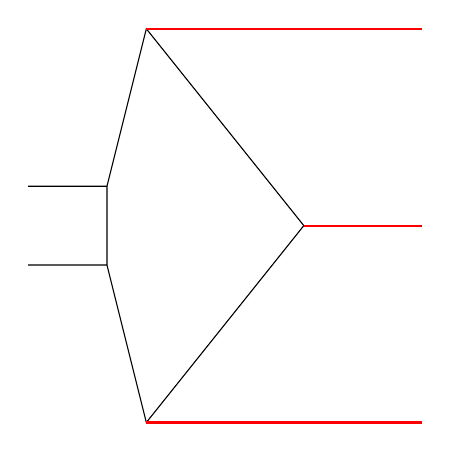
\begin{tikzpicture}[scale = 0.5]
\draw 	(0,4) -> (2,4) -> (2,6) -> (0,6)
		(2,4) -> (3,0) -> (7,5) -> (3,10) -> (2,6);
\draw [red, thick]	(3,0) -> (10,0)
					(7,5) -> (10,5)
					(3,10) -> (10,10);
\end{tikzpicture}\\
Die drei roten Kanten ersetzen die ehemaligen Kanten von $v$.
\end{center}

%% 26.05.15, 8.VL
\section{$st$-Flüsse}
\subsection{Definition: $st$-Fluss}
Seien folgende Dinge gegeben
\begin{itemize}
\item $G$ symmetrischer gerichteter Graph, $\rev{a \pfeil b } := b \pfeil a$
\item $c : E \pfeil \R$ Kapazitätsfunktion
\item $s,t \in V$
\end{itemize}
Ein \df{$st$-Fluss} ist eine Abbildung $\phi : E \pfeil \R$, s.d.
\begin{itemize}
\item $\phi(e) = - \phi ( \rev{e})$
\item $\forall w \in V-\{s,t\} :~~\sum_{v \in V} \phi(v \pfeil w) = 0$ 
\end{itemize}
$\phi$ heißt \df{zulässig}, falls $\phi \leq c$.

\subsection{Parametrisches Kürzeste-Wege-Problem}
\paragraph{Gegeben}
\begin{itemize}
\item  $G = (V,E)$ ein gerichteter Graph
\item $E' \subset E$
\item  $c : E\pfeil \R$ und
\begin{align*}
c(\lambda, e ) := 
\left\lbrace
\begin{aligned}
 c(e) - \lambda && e \in E'\\
 c(e) && e \notin E
\end{aligned}
\right.
\end{align*}
\end{itemize}
\paragraph{Gesucht} Größtes $\lambda$, sodass $G$ bzgl. $c(\lambda, \cdot)$ keine negativen Kreise enthält.
\paragraph{Laufzeit} $\O{n^2\log n}$ bzw. $\O{nm\log n}$

\subsection{Definition}
Ein \df{gerichteter $st$-Schnitt} ist eine Kantenmenge $C$, sodass jeder $st$-Pfad nichttrivialen Schnitt mit $C$ hat.

\subsection{Dualität}
$C$ gerichteter $st$-Schnitt $\Longleftrightarrow$ $C^*$ gerichteter Kreis, der $s^*$ und $t^*$ trennt.

\subsection{Definition}
$C$ heißt \df{Kozykel}, falls $C^*$ ein einfacher gerichteter Kreis ist.

\subsection{Lemma}
Sei $\pi: E \pfeil \R$ der \df{Einheitsfluss} eines einfachen $st$-Pfades $P$, d.h.
\begin{align*}
\pi(e) :=
\left\lbrace
\begin{aligned}
1 && e\in P\\
-1 && \rev{e} \in P\\
0 && \text{sonst}
\end{aligned}
\right.
\end{align*}
Dann gilt für jeden Kozykel $C$: $\pi(C) \in \{-1,0,1\}$.\\
Ferner: $\pi(C) = 1 \Longleftrightarrow C$ ist $(s,t)$-Schnitt

\paragraph{Beweis}
\begin{enumerate}
	\item[Fall 1:] $s,t$ liegen auf derselben Seite von $C^*$
	\begin{align*}
	\Longleftrightarrow & P \text{ kreuzt } C^* \text{ gleich oft in jeder Richtung}\\
	\Longleftrightarrow & C \text{ enthält dieselbe Zahl von Kanten in }P \text{ und }\overline{P}\\
	\Longleftrightarrow & \pi(C) = 0
	\end{align*}
		\item[Fall 2:] $s$ liegt innen und $t$ außen von $C^*$
		\begin{align*}
		\Longleftrightarrow & P \text{ kreuzt } C^* \text{ einmal mehr in die Richtung von }s\rightarrow t\\
		\Longleftrightarrow & C \text{ enthält eine Kante mehr in }P \text{ als in }\overline{P}\\
		\Longleftrightarrow & \pi(C) = 1
		\end{align*}
			\item[Fall 2:] $s$ liegt innen und $t$ außen von $C^*$\\
			analog wie Fall 2
\end{enumerate}

\subsection{Definition}
Setze $\phi = \lambda \cdot \pi$. Das \df{Residual-Netzwerk} $G_\lambda$ ist definiert als $G$ mit Kapazitätsfunktion
\[ c(\lambda, e) = c(e) - \lambda \cdot \pi(e) \]
Definiere $G_\lambda^*$ als $G^*$ mit Kapazitätsfunktion
\[ c(\lambda, e^*) = c(\lambda, e) \]

\subsection{Lemma}
$G$ besitzt einen gültigen $s-t$-Fluss mit Wert $\lambda$ genau dann, wenn $G^*_\lambda$ keinen negativen Kreis enthält.

\paragraph{Beweis}
Zeige '$\Longrightarrow$': Annahme: $G^*_\lambda$ enthält negativen Kreis $C^*$, d.h.
$0 >c(\lambda, C^*) = \sum_{e \in C}c(\lambda,e)= \sum_{e\in C}c(e) - \lambda \sum_{e\in C}\pi(e) = c(C) - \lambda \pi(C)$
$\Longrightarrow \pi(C)  > c(C)/ \lambda \leq 0 \Longrightarrow \pi(C) = 1$
\[\Longrightarrow C \text{ ist } s-t-\text{Schnitt}\]
Außerdem $c(C) < \lambda$, d.h. es existiert ein Schnitt mit Kapazität $< \lambda$, das ist ein Widerspruch

Zeige '$\Longrightarrow$': $G_\lambda^*$ enthält keinen negativen Kreis.\\
$\Longrightarrow$ kürzeste Wege wohldefiniert;
sei $x$ in $G^*_\lambda$ beliebiger Ursprung, $dist(p,\lambda) := $ Distanz von $x$ zu $p$

\paragraph{Definition}
\[\phi(\lambda, e) := dist(\lambda, head(e^*)) - dist(\lambda, tail(e^*)) + \lambda \pi(e) \]
wobei
\[ dist(\lambda, p) := \min c(\lambda, o \pfeil^* p) \]
wobei $o \in G^*$ beliebig, aber fest.\\

Zeige $\phi$ ist gütliger $st$-Fluss
\begin{enumerate}
	\item Für $v \in V$ gilt: $\sum_{w}\phi(v \rightarrow w) = \sum_{w}\lambda \pi(v \rightarrow w)$
	es folgt: $\phi(\lambda, \cdot)$ ist Fluss mit Wert $\lambda$
	\item $slack(\lambda, e^*) := dist(\lambda, tail(e^*)) + c(\lambda, e) - dist(\lambda, head(e^*)) $
	es gilt: $slack(\lambda, e) = c(e) - \phi(\lambda, e)$
	$\phi(\lambda, e) \leq c(e) \Longleftrightarrow slack(\lambda, e) \geq 0$
	Wäre $slack(\lambda, e) < 0$, dann folgt: $dist(\lambda, head(e^*)) > dist(\lambda, tail(e^*)) + c(\lambda, e^*)$, das wäre ein Widerspruch
\end{enumerate}

\subsection{Satz}
Ein maximaler $st$-Fluss in einem $st$-planaren Graphen kann in $\O{n\log n}$ berechnet werden.

\subsection{Definition}
Ein Graph heißt $st$-planar, falls er so planar eingebettet werden kann, dass $s$ und $t$ an der selben Facette liegen.

\subsection{Satz}
Ein maximaler $st$-Fluss in einem $st$-planaren Graph kann in $\O{n\log n}$ Zeit berechnet werden.

Max $\lambda$, s.d. kein neg. Kreis in $G^*_\lambda$ ist Länge des kürzesten $ts$-Weges in $G^*_\lambda$

%% 27.05.15 9. VL
\newpage
\section{Das Menger-Problem}

\subsection{Zur Erinnerung}
$S \subset V$ heißt Separator in $G$, falls $G - S$ unzusammenhängend.\\
$S\subset E$ heißt Schnitt in $G$, falls $G - S$ unzusammenhängend.


\subsection{Definitionen}
Zu $u,v \in V$ definiere den \df{Knotenzusammenhang}
\begin{align*}
\kappa_G(u,v) := \left\lbrace \begin{aligned}
|V| - 1, \text{ falls }\{u,v\} \in E\\
\min_{S\subset V}|S|, \text{ für } S \text{ Separator, der u und v trennt}
\end{aligned} \right.
\end{align*}
und $\kappa_G := \min_{u,v\in V}\kappa_G(u,v)$

\[\lambda_G(u,v) := \min_{S \subset E, \text{ S Schnitt und trennt u und v}}|S| \]
und
\[\lambda(G) := \min_{u,v\in V} \lambda_G(u,v) \]

Zwei Wege heißen \df{kantendisjunkt}, wenn sie keine gemeinsame Kante enthalten, und (intern) \df{knotendisjunkt}, wenn sie außer Anfangs- und Endknoten keinen gemeinsamen Knoten enthalten.

\subsection{Satz von Menger}
Seien $s$ und $t$ Knoten in $G = (V,E)$
\begin{itemize}
\item Sei $\{s,t\}\notin E$, dann existieren genau $\kappa_G(s,t)$ knotendisjunkte $st$-Wege.
\item Es existieren genau $\lambda_G(s,t)$ kantendisjunkte $st$-Wege.
\end{itemize}

\subsection{Menger-Problem}
Finde zu $G,s,t$ maximale Anzahl knotendisjunkter bzw. kantendisjunkter $st$-Wege.

\subsection{Menger-Problem in planaren Graphen: kantendisjunkte Variante}
Linearzeitalgorithmus basierend auf \textsc{Right-First-DFS}.

\paragraph{Spezialfall}
$s$ und $t$ liegen auf derselben Facette:\\
\textsc{Right-First} $=$ im Gegenuhrzeigersinn nächste freie Kante in Adjazenzliste (relativ zur aktuellen eingehenden Kante).

\paragraph{Algorithmus}
$G$ planar eingebetteter Graph, OE $t$ auf äußerer Facette
\begin{enumerate}
	\item Ersetze $G$ durch den gerichteten Graphen $\overrightarrow{G}$, indem $\{u,v\} \in E$ durch $(u,v)$ und $(v,u)$ ersetzt wird. (in $\O{n}$)
	\item Berechne in $\O{n}$ Menge gerichteter einfacher kantendisjunkter Kreise $\overrightarrow{C_1},\ldots, \overrightarrow{C_l}$ und konstruiere aus $\overrightarrow{G}$ den Graphen $\overrightarrow{G}_C$, indem die Richtung aller Kanten auf den $\overrightarrow{C_i}$ umgedreht wird.
	\item Berechne in $\overrightarrow{G}_C$ in $\O{n}$ mittels \textsc{Right-First-DFS} eine maximale Anzahl kantendisjunkter gerichteter $st$-Wege.
	\item Berechne aus den in Schritt 3 gefundenen $st$-Wegen in $\overrightarrow{G}_C$ gleiche Anzahl kantendisjunkter $st$-Wege in $G$ in $\O{n}$.
\end{enumerate}

\paragraph{Schritt 1}
\paragraph{Lemma}
Seien $P_1, \ldots, P_r$ kantendisjunkte, gerichtete $st$-Wege in $\overrightarrow{G}$. Dann enthält
\[P = \set{\{u,v\} \in E}{\text{Genau eine der Kanten (u,v) und (v,u) liegt auf einem der }P_i}\]
gerade $r$ kantendisjunkte $st$-Wege in $G$.

\paragraph{Beweis}
Zwei Fälle: Wir konstruieren in beiden Fällen aus gegebenen $st$-Wegen unproblematische $st$-Wege
\begin{enumerate}
	\item $(u,v) \in P_i \wedge (v,u) \in P_i$: Entferne $(u, v, \ldots, v, u)$ bzw. $(v, u, \ldots, u, v)$ aus $P_i$
	\item $(u,v) \in P_i \wedge (v,u) \in P_j$: $P_i = (A, u, v, B)$, $P_j = (C, v, u, D)$; konstruiere $\widetilde{P}_i = (A, D)$ und $\widetilde{P}_j = (C, B)$
\end{enumerate}

\paragraph{Schritt 2}
$C_1,\ldots, C_l$ in $\overrightarrow{G}$, sodass
\begin{enumerate}
	\item $\overrightarrow{G}_C$ enthält keine Rechtskreise, d.h. keine Kreise, deren Inneres rechts liegt (aus Sicht einer Kante).
	\item Sei $\overrightarrow{P}_C \subset \overrightarrow{E}_C$ Menge der Kanten auf kantendisj. $s-t$ Wegen in $\overrightarrow{G}_C$ und $\overrightarrow{P} \subset \overrightarrow{E}$, wobei
	\[\overrightarrow{P} := (\overrightarrow{P}_C \cap \overrightarrow{E})\cup \{(u,v) \in \overrightarrow{E}: (u,v) \text{ auf einem der }\overrightarrow{C}_i \text{ und } (v,u)' \notin \overrightarrow{P}_C \} \]
	Dann induziert $\overrightarrow{P}$ $k$ kantendisjunkte gerichtete $st$-Wege in $\overrightarrow{G}$ g.d.w $\overrightarrow{P}_C$ induziert $k$ kantendisjunkte gerichtete $st$-Wege in $\overrightarrow{G}_C$.
\end{enumerate}

\paragraph{Konstruktion der Kreise $C_1, \ldots, C_l$}
Sei $f$ Facette in $G$ bzw. $\overrightarrow{G}$; definiere Abstand von $f$ zur äußerer Facette $f_0$ als
\[dist(f) := \text{Länge eines kürzesten Weges des Dualknotens }f^* \text{ zum Dualknoten der äußeren Facette }f_0^* \text{ in }G^*\]
Definiere $C_i$ als Vereinigung der einfachen Kreise in $G$ für die alle Facetten $f$ im Inneren die Bedingung $dist(f) \geq i$ erfüllen. $\overrightarrow{C}_i$ sei entsprechender Rechtskreis in $\overrightarrow{G}$.
Drehe alle diese $C_i$ um, erhalte $\overrightarrow{G}_C$.\\


%%3.6.15, 10.VL
$\overrightarrow{G}_C$ enthält keine Rechtskreise, da für jeden Rechtskreis in $\overrightarrow{G}$ beim Übergang zu $\overrightarrow{G}_C$ mindestens eine Kante des Kreises umgedreht wird.\\\\

Sei $\overrightarrow{P}_C \subset \overrightarrow{E}_C$ Kantenmenge zu $k$ $st$-Wegen in $\overrightarrow{G}_C$. Konstruiere dazu Kantenmenge $\overrightarrow{P}$ in $\overrightarrow{G}$.
\[\overrightarrow{P} := (\overrightarrow{P}_C \cap \overrightarrow{E})\cup
\{(u,v) \in \overrightarrow{E}: (u,v) \text{ auf einem }\overrightarrow{C}_j \text{ und }(v,u)' \notin \overrightarrow{P}_C \}
\]

\paragraph{Schritt 3}
Berechnung einer maximalen Anzahl kantendisjunkter $st$-Wege in $\overrightarrow{G}_C$(in $\O{n}$)\\
Schleife über ausgehende Kanten aus $s$\\
\textsc{RightFirstDepthSearch}:\\
Suchschritt: rechteste nicht markierte auslaufende Kante in Bezug auf Referenzkante\\\\

Zwei Variationen, wie die \df{Referenzkante} zu wählen ist
\begin{enumerate}
	\item Weihe: aktuell einlaufende Kante
	\item Coupry: erste einlaufende Kante
\end{enumerate}

\paragraph{Korrektheitsbeweis zu Schritt 3}
Beh.: $\overrightarrow{P}_C$ enthält maximale Anzahl kantendisjunkter $st$-Wegen.\\
Benutze dazu gewichtete Variante des Satz v. Menger, d.h. konstruiere $st$-Schnitt der entsprechenden Kapazität.\\
Schnitt A wird induziert durch geeigneten Kreis $\overrightarrow{K} \subset \overbrace{G}_C$ mit:
\begin{enumerate}
	\item $s\in Innen(\overrightarrow{K})$ oder auf $\overrightarrow{K}$
	\item $t \in Aussen(\overrightarrow{K})$
	\item $A :=\set{(u,v)\in \overrightarrow{E}_C}{u \text{ liegt auf }\overrightarrow{K}, v \in Aussen(\overrightarrow{K})}$, $|A| = $\# $st$-Wegen in $\overrightarrow{P}_C$
\end{enumerate}

$\overrightarrow{K}$ wird mittels \textsc{LeftFirst}-Rückwärtssuche von $s$ aus in $\overrightarrow{P}_C$ konstruiert.\\
Wie sieht $\overrightarrow{K}$ aus:
\paragraph{Variante 1}
$\overrightarrow{K}$ geht von $s$ nach $s$
\paragraph{Variante 2}
$\overrightarrow{K}$ geht von $s \neq v_0$ nach $v_0$ und $s$\\
In diesem Fall den Kreis, der von $v_0$ nach $v_0$ beschrieben wird.

\subsection{Lemma}
Betrachte $\overrightarrow{G}_C = (V,\overrightarrow{E}_C)$ und $\overrightarrow{K}$, dann ist jede Kante $(u,v) \in \overrightarrow{E}_C$ mit $u$ auf $\overrightarrow{K}$ und $v \in Aussen(\overrightarrow{K})$ durch einen $st$-Weg aus $\overrightarrow{P}_C$ besetzt.

\paragraph{Beweis}
\begin{enumerate}
	\item Wenn $P_1,\ldots, P_l$ $st$-Wege sind und $\overrightarrow{K}$ ein Linkskreis von $s$ nach $s$, dann gehört keine der Kanten $(x,y)$, $x \in Aussen(\overrightarrow{K}), y \in \overrightarrow{K}$ zu einem der $p_i$.\\
	Wegen \textsc{LeftFirst} in Graph indziert durch $p_1,\ldots, p_l$ $(x,y) \in p_i$, für alle $1 \leq i \leq l$.\\
	Deswegen: Kante $(u,v)$ mit $u$ auf $\overrightarrow{K}$, $v \in Aussen(\overrightarrow{K})$ kann nicht auf einem Linkskreis aus $p_1,\ldots, P_l$ liegen.
	
	\item betrachte $(u,v)$ mit $u$ auf $\overrightarrow{K}$, $v \in Aussen(\overrightarrow{K})$ und $(u,w)$ mit $w$ auf $\overrightarrow{K}$.\\
	Annahme: $(u,v)$ gehört zu keinem der $P_1, \ldots, P_l$.\\
	Betrachte Referenzkante zu $(u,w)$ in \textsc{RightFirst}-Suche (Schritt 3)\\
	Referenzkante geht von Innerem zum Kreis oder liegt auf den Kreis,\\
	aber dann hätte \textsc{RightFirst} nicht $(u,w)$ sondern $(u,v)$ gewählt. Das wäre ein Widerspruch.
\end{enumerate}

%% 16.06.15, 12.VL

\section{Das Okamura \& Seymour Problem}
Sei $G$ ein planarer Graph, $D = \{\{s_i,t_i\}, s_i,t_i \in V, 1 \leq i \leq k \}$, $s_i, t_i$ liegen alle auf Rand der äußeren Facette.\\
Finde $k$ paarweise kantendisjunkte Wege, die jeweils $s_i$ mit $t_i$ verbinden.

\subsection{Kapazitätsbedingung}
Für jeden Schnitt $X \subset V$ ist die \df{freie Kapazität} $fcap(X) \geq 0$,
\[fcap(X) := cap(X) - dens (X)\]
\[cap(X) = \left|\set{\{x,y\} \in E}{x \in X, y \in V\setminus X}\right|\]
\[dens(X) = \left|\set{\{s,t\} \in D}{\#(\{s,t\}\cap X) = 1}\right|\]
(\df{Kapazität} und \df{Dichte} von $X$)\\
Die Kapazitätsbedingung ist offensichtlich notwendig für Lösbarkeit des Problems. Allerdings ist sie i.A. nicht hinreichend.

\paragraph{Anti-Beispiel}
Ein Quadrat, mit den Ecken $a,b,c,d$ mit Farben 1,2,1,2. Erfüllt Kapazitätsbedingung, löst aber Problem nicht. $fcap(X) = 1$, wobei $X = \set{a}{}$.

\subsection{Geradheitsbedingung}
Für alle Schnitte $X \subset V$ gilt $fcap(X)$ ist gerade.

\subsection{Satz von Okamura \& Seymour}
Falls die Geradheitsbedingung erfüllt ist, ist die Kapazitätsbedingung äquivalent zur Lösbarkeit des Problems.

\subsection{Lemma}
Es gilt:
\[fcap(X) \text{ gerade }\forall X \subset V \Longleftrightarrow fcap(v) \text{ gerade }\forall v \in V \]
wobei
\[fcap(v) = d(v) - dens(v) \]
\[dens(v) = \# \set{i }{s_i = v} + \# \set{i }{t_i = v}\]

\paragraph{Beweis}
$\Longrightarrow$ trivial.\\
$\Longleftarrow$: Sei $fcap(v)$ gerade für alle $v$, $X \subset V$:\\
\[cap(X) = \sum_{v\in X} cap(v) - 2 \left|\set{\{u,v\} \in E}{u,v \in X}\right|\]
\[dens(X) = \sum_{v\in X}dens(v) - 2 \left|\set{\{s,t\} \in D}{s,t \in X}\right| \]
\[fcap(X) = \sum_{v\in X} cap(v) - \sum_{v\in X} dens(v) - 2 \left|\set{\{u,v\} \in E}{u,v \in X}\right| + 2 \left|\set{\{s,t\} \in D}{s,t \in X}\right|
 = \sum_{v\in V}fcap(v) - 2 N \in 2\Z \]
 $N \in \N$\qed

\subsection{Linearzeitalgorithmus für planaren Graphen $G$}
Terminalpaare $D$ auf äußerer Facette und Geradheitsbedingung erfüllt.\\

\begin{enumerate}
	\item[Phase 1] Konstruiere aus $G, D$ einfachere Instanz mit Klammerstruktur und berechne mittels \textsc{RightFirst}-Tiefensuche kantendisjunkte Lösungswege $q_1, \ldots, q_k$. Diese induzieren gerichteten Hilfsgraph.
	\item[Phase 2] Berechne mittels gerichteter \textsc{RightFirst}-Tiefensuche in Hilfsgraph Lösungswege $p_1,\ldots, p_k$, die jeweils $s_i$ mit $t_i$ verbinden.
\end{enumerate}

\subsection{Phase 1: Instanz mit Klammerstruktur}
$G, D = \set{\{s_i,t_i\}}{}$
\begin{enumerate}
	\item Wähle beliebiges Terminal als Startterminal.
	\item Gehe im Gegenuhrzeigersinn: Dem ersten Terminal eines Paares, das einem begegnet, ordnet man ein aufgehende Klammer zu. Begegnet man dem zweiten, erhält dieses eine zugehende Klammer.\\
	Entsprechende Klammerpaare ergeben neue Terminalpaare in $D'$ (innere Klammerpaare haben kleineren Index).
	\item Konstruiere mittels \textsc{RightFirst}-Suche Lösung $q_1,\ldots, q_k$ zu $G$, $D'$; Reihenfolge, in der Wege berechnet werden nach Reihenfolge der $t_i'$, d.h. von innen nach außen in Klammerstruktur.
\end{enumerate}

\subsection{Korrektheit von Phase 1}
\paragraph{Beobachtung} 
\begin{enumerate}
	\item keine zwei Wege $q_i, q_j$ kreuzen sich, wg. \textsc{RightFirst}-Auswahlregel
	\item kein $q_i$ kreuzt sich selbst
	\item Sei $G'$ der gerichtete Graph, der durch die $q_i$ induziert wird. $G'$ enthält keinen Rechtskreis.\\
	Angenommen $G'$ hätte einen Rechtskreis, dann wären an diesem mind. zwei $q_i, q_j$ beteiligt. Daraus folgt auf der Facette folgende Terminale: $s_i, t_j, s_j, t_i$, was der Klammerung $()()$ entspricht, was ein Widerspruch zur Paarung ist.\\
	\item 1, 2 \& 3 $\Longrightarrow$ induktiv über $q_i$ kann gezeigt werden, dass $q_i$ die richtigen Terminale verbindet.
	\item 1.Phase in $\O{n}$ klar.
\end{enumerate}

%%% 17.6.15, 13.VL

\subsection{Phase 2}
Ohne Einschränkung sei von Startterminal im Gegenuhrzeigersinn jeweils $s_i$ vor $t_i$ und Indizierung entsprechend Auftreten der $t_i$.\\
Für $i = 1, \ldots, k$
\begin{enumerate}
	\item $p_i := $ führe \textsc{RFS} in $G'$ von $s_i$ aus bis zu einem $j$
	\item Falls $i \neq j$, \textsc{Stop}.
\end{enumerate}
gebe $p_1,\ldots, p_k$ aus.

\paragraph{Laufzeit}
$\O{n}$ amortisiert mit \textsc{Union-Find} wie beim kantendisjunkten Menger-Problem.

\paragraph{Korrektheit}
Der Algorithmus endet entweder
\begin{enumerate}
	\item mit Wegen $p_1,\ldots, p_k$, die jeweils $s_i$ mit $t_i$ verbinden.
	\item $p_1,\ldots, p_{i-1}$ korrekt und $p_i$ verbindet $s_i$ mit $t_j$\\
	$\Longrightarrow i < j$, da $i \neq j$\\
	Prozedur, die Weg $p$ berechnet, so dass $p$ einen Schnitt $X$ induziert, der im Fall 1 \df{saturiert} ist, d.h. $fcap(X) = $ und der im Fall 2 \df{übersaturiert} ist, d.h. $fcap(X) < 0$.
\end{enumerate}

\paragraph{Prozedur} für Schnitt $X$:\\
Rückwärts-\textsc{LFS} startet von Terminal $t_i$ bzw. $t_j$ wo Weg $p_i$ endet in Graph, der durch $p_1,\ldots, p_i$ induziert wird.

\subsection{Lemma}
Sei $A$ Menge der Kanten $\{u,v\}$ aus $G$ mit $u$ auf $p$ und $v$ rechts von $p$. Jede Kante $\{u,v\} \in A$ gehört zu $G'$ und genau dann in Orientierung $(u,v)$, wenn sie durch eine der $p_1, \ldots, p_i$ besetzt ist.

\paragraph{Beweis}
Wenn $\{u,v\}$ durch ein $p_i$ besetzt, dann wegen Konstruktion von $p$ in Orientierung $(u,v)$.
\begin{enumerate}
	\item[Fall 1] Es existiere $(u,v)$ mit $(u,v)$ nicht durch $p_1, \ldots, p_i$ besetzt. Mein Bild zeigt einen Widerspruch zu RFS Ur argument is invalid.
	\item[Fall 2] Es existiert $\{u,v\} \in A, (u,v), (v,u) \notin G'$. Bild. ICh bin müde as fuck\ldots
	\qed
\end{enumerate}

\subsection{Lemma}
Sei $X$ Schnitt induziert durch $p$ (Knoten rechts von $p$). Falls $p_i$ $s_i-t_i$-Weg, so ist $fcap(X) = 0$, sonst $fcap(X) < 0$.
\paragraph{Beweis}
Kanten $\{u,v\}$ auf $p$, $v$ rechts von $p$ entweder zu Weg $p_j$ gehört mit $1 \leq j < i, s_j \in V\setminus X$ und $t_j\in X$ oder zu Weg $q_j$ aus erster Phase mit $s_j'\in X$ und $t_j' \in V\setminus X$.\\
Wenn $p_i$ korrekter $s_i-t_i$-Weg, so gilt
\[cap(X) = \# \set{\{s_j, t_j\}}{s_j \notin X, t_j \in X, 1 \leq j \leq l}
+\# \set{\{s_j', t_j'\}}{s_j' \in X, t_j' \notin X, \{s_i', t_j'\} \notin D } \]
\[ = dens(X)\]
Wenn $p_i$ nicht korrekt, d.h. $s_i$ mit $t_j$, $i< j$, verbindet, so ist $cap(X) < dens(X)$, da $s_i \notin X, t_i \in X$.
\qed



\end{document}